\documentclass[11pt, hyperref={pdfpagelabels=true}]{beamer}
%\usepackage{etex} % math fonts misbehave
\usepackage{lmodern} 
%\usefonttheme{structurebold}

\usepackage{gauss}
\usepackage{amsmath}
\usepackage{amsfonts}
\usepackage{lipsum}
\usepackage{graphicx}
\usepackage{subfigure}
\usepackage{setspace}
\usepackage{amssymb}
\usepackage{multirow}
\usepackage{xcolor}
\usepackage{ragged2e}
\usepackage{mathrsfs}
\usepackage{courier}
\usepackage{diagbox}
%\usepackage{bbold} % missing 11pt
\usepackage[all]{xy}

\setbeamertemplate{footline}[frame number]
\setbeamercolor{normal text}{bg=white!10}
\setbeamertemplate{theorems}[numbered]

\newcommand{\C}{\mathbb{C}} 
\newcommand{\F}{\mathbb{F}} 
\newcommand{\R}{\mathbb{R}} 
\newcommand{\Q}{\mathbb{Q}}
\newcommand{\N}{\mathbb{N}}
\newcommand{\Z}{\mathbb{Z}}

\newcommand{\HRule}{\rule{\linewidth}{0.5mm}}
\newcommand{\U}{\mathsf}
\newcommand{\celsius}{\ensuremath{^{\circ}\mathsf{C}}}
\newcommand{\myseries}[2]{#1_1,\ldots,#1_{#2}}
\newcommand{\highlightr}[1]{\textcolor[rgb]{1,0.3,0.2}{\emph{\textbf{#1}}}}
\newcommand{\highlightg}[1]{\textcolor[rgb]{0.1,0.5,0.3}{\emph{\textbf{#1}}}}
\newcommand{\structb}[1]{\textcolor[rgb]{0.2,0.2,0.7}{#1}}
\newcommand{\red}[1]{\textcolor[rgb]{1,0,0}{#1}}
\newcommand{\bemph}[1]{\emph{\textbf{#1}}}
\newcommand{\tabincell}[2]{\begin{tabular}{@{}#1@{}}#2\end{tabular}}

\renewcommand\arraystretch{1.8}


\title{VE401 Probabilistic Methods in Eng. \\RC 6}
\author{CHEN Xiwen} 
\date{\today} 
\institute[UM-JI]{UM-SJTU Joint Institute}


\AtBeginSubsection[]{
\begin{frame}
\tableofcontents[sectionstyle=show/shaded,subsectionstyle=show/shaded]
\end{frame}
}

\begin{document}



\begin{frame}
\titlepage
\end{frame} 


\begin{frame}
\frametitle{Table of contents}
\tableofcontents
\end{frame} 

\section{Test for Statistics}

\subsection{Comparison of Two Means}

\begin{frame}{Comparing Two Means}

\justifying
\structb{Basic distribution.} Suppose sample means $\overline{X}^{(1)}$ and $\overline{X}^{(2)}$ are cal-culated from samples of sizes $n_1$ and $n_2$ respectively from normal populations with means $\mu_1, \mu_2$ and variances $\sigma_1, \sigma_2$. Then since
\begin{align*}
\overline{X}^{(1)}\sim \U{N}(\mu_1, \sigma_1^2/n_1), \qquad \overline{X}^{(2)} \sim \U{N}(\mu_2, \sigma_2^2/n_2),
\end{align*}
the statistic
\begin{align*}
Z = \frac{\overline{X}^{(1)} - \overline{X}^{(2)} - (\mu_1 - \mu_2)}{\sqrt{\sigma_1^2/n_1 + \sigma_2^2/n_2}}
\end{align*}
follows a standard normal distribution.

\end{frame}


\begin{frame}{Variances Known}

\justifying
\structb{Variances known.} Let $X_1^{(i)}, \ldots, X_{n_i}^{(i)}$ with $i = 1, 2$ be samples of sizes $n_1$ and $n_2$ from normal distributions with unknown means $\mu_1, \mu_2$ and \highlightr{known} variances $\sigma_1^2, \sigma_2^2$. Then the test statistic is given by
\begin{align*}
Z = \frac{\overline{X}^{(1)} - \overline{X}^{(2)} - (\mu_1 - \mu_2)_0}{\sqrt{\sigma_1^2/n_1 + \sigma_2^2/n_2}}
\end{align*}
We reject at significance level $\alpha$
\begin{itemize}
	\item $H_0: \mu_1 - \mu_2 = (\mu_1-\mu_2)_0$ if $|Z| > z_{\alpha/2}$,
	\item $H_0: \mu_1 - \mu_2 \leq (\mu_1-\mu_2)_0$ if $Z > z_{\alpha}$,
	\item $H_0: \mu_1 - \mu_2 \geq (\mu_1-\mu_2)_0$ if $Z < -z_{\alpha}$.
\end{itemize}

\end{frame}


\begin{frame}{Variances Known}

\justifying
\structb{OC curve.} When testing equality of means $H_0: \mu_1 = \mu_2$, we have $(\mu_1-\mu_2)_0 = 0$. We can use the OC curves for normal distributions with
\begin{align*}
d = \frac{|\mu_1-\mu_2|}{\sqrt{\sigma_1^2+\sigma_2^2}}
\end{align*}
with $n = n_1 = n_2$. When $n_1\neq n_2$, we use the equivalent sample size
\begin{align*}
n = \frac{\sigma_1^2 + \sigma_2^2}{\sigma_1^2/n_1 + \sigma_2^2/n_2}.
\end{align*}

\end{frame}

\begin{frame}{Variances Equal but Unknown --- Student's $T$-Test}

\justifying
\structb{Variances equal but unknown.} Let $X_1^{(i)}, \ldots, X_{n_i}^{(i)}$ with $i = 1, 2$ be samples of sizes $n_1$ and $n_2$ from normal distributions with unknown means $\mu_1, \mu_2$ and \highlightr{equal} but \highlightr{unknown} variances $\sigma^2 = \sigma_1^2 = \sigma_2^2$. Then the test statistic is given by
\footnotesize
\begin{align*}
T_{n_1+n_2-2} = \frac{\overline{X}^{(1)} - \overline{X}^{(2)} - (\mu_1-\mu_2)_0}{\sqrt{S_p^2(1/n_1+1/n_2)}},
\end{align*}
\normalsize
with \highlightg{pooled estimator for variance}
\footnotesize
\begin{align*}
S_p^2 = \frac{(n_1-1)S_1^2 + (n_2-1)S_2^2}{n_1+n_2-2}.
\end{align*}
\normalsize
We reject at significance level $\alpha$
\begin{itemize}
	\item $H_0: \mu_1 - \mu_2 = (\mu_1-\mu_2)_0$ if $|T_{n_1+n_2-2}| > t_{\alpha/2, n_1+n_2-2}$,
	\item $H_0: \mu_1 - \mu_2 \leq (\mu_1-\mu_2)_0$ if $T_{n_1+n_2-2} > t_{\alpha,n_1+n_2-2}$,
	\item $H_0: \mu_1 - \mu_2 \geq (\mu_1-\mu_2)_0$ if $T_{n_1+n_2-2} < -t_{\alpha,n_1+n_2-2}$.
\end{itemize}

\end{frame}


\begin{frame}{Variances Equal but Unknown --- Student's $T$-Test}

\justifying
\structb{OC curve.} When testing equality of means $H_0: \mu_1 = \mu_2$, we have $(\mu_1-\mu_2)_0 = 0$. We can use the OC curves for the T-test in case of equal sample sizes $n = n_1 = n_2$
\begin{align*}
d = \frac{|\mu_1-\mu_2|}{2\sigma}.
\end{align*}
When reading the charts, we must use the modified sample size $n^* = 2n-1$.

\end{frame}


\begin{frame}{Variances Unequal and Unknown --- Welch's $T$-test}

\justifying
\structb{Welch-Satterthwaite Relation.} Let $X^{(1)}, \ldots, X^{(k)}$ be $k$ independent normally distributed random variables with variances $\sigma_1^2, \ldots, \sigma_k^2$. Let $s_1^2, \ldots, s_k^2$ be sample variances based on samples of sizes $n_1, \ldots, n_k$ from the $k$ populations, respectively. Let $\lambda_1, \ldots, \lambda_k > 0$ be positive real numbers and define
\begin{align*}
\gamma := \frac{(\lambda_1 s_1^2 + \cdots + \lambda_k s_k^2)^2}{\displaystyle\sum_{i=1}^k \dfrac{(\lambda_i s_i^2)^2}{n_i-1} }.
\end{align*}
Then
\begin{align*}
\chi_{\gamma}^2 := \gamma \cdot \frac{\lambda_1 s_1^2 + \cdots + \lambda_k s_k^2}{\lambda_1 \sigma_1^2 + \cdots + \lambda_k \sigma_k^2}
\end{align*}
follows approximately a chi-squared distribution with $\gamma$ degrees of freedom, where we round $\gamma$ \highlightr{down} to the nearest integer.


\end{frame}


\begin{frame}{Variances Unequal and Unknown --- Welch's $T$-test}

\justifying
\structb{Welch's T-test.} Let $X_1^{(i)}, \ldots, X_{n_i}^{(i)}$ with $i = 1, 2$ be samples of sizes $n_1$ and $n_2$ from normal distributions with unknown means $\mu_1, \mu_2$ and \highlightr{unequal} and \highlightr{unknown} variances $\sigma_1^2, \sigma_2^2$. The test statistic is given by
\begin{align*}
T_{\gamma} = \frac{\overline{X}^{(1)} - \overline{X}^{(2)} - (\mu_1-\mu_2)_0}{\sqrt{S_1^2/n_1 + S_2^2/n_2}}, \qquad \gamma = \frac{(S_1^2/n_1 + S_2^2/n_2)^2}{\dfrac{(S_1^2/n_1)^2}{n_1-1} + \dfrac{(S_2^2/n_2)^2}{n_2-1}}
\end{align*}
We reject at significance level $\alpha$
\begin{itemize}
	\item $H_0: \mu_1-\mu_2 = (\mu_1-\mu_2)_0$ if $T_{\gamma} > t_{\alpha/2,\gamma}$,
	\item $H_0: \mu_1-\mu_2 \leq (\mu_1-\mu_2)_0$ if $T_{\gamma} > t_{\alpha,\gamma}$,
	\item $H_0: \mu_1-\mu_2 \geq (\mu_1-\mu_2)_0$ if $T_{\gamma} < -t_{\alpha,\gamma}$.
\end{itemize}



\end{frame}


\subsection{Non-parametric Comparisons}


\begin{frame}{Wilcoxon Rank-Sum Test}

\justifying
\structb{Wilcoxon rank-sum test.} Let $X$ and $Y$ be two random populations following some continuous distributions. \\
~\\
Let $X_1, \ldots, X_m$ and $Y_1, \ldots, Y_n$, where $m\leq n$, be random samples from $X$ and $Y$ and associate the rank $R_i, i = 1,\ldots, m+n$, to the $R_i$th smallest among the $m+n$ total observations. If ties in the rank occur, the mean of the ranks is assigned to all equal values. The test statistic is given by
\begin{align*}
W_m = \U{sum\ of\ the\ ranks\ of\ } X_1, \ldots, X_m
\end{align*}
We reject $H_0: P[X > Y] = 1/2$ at significance level $\alpha$ if $W_m$ falls into the corresponding critical region. 


\end{frame}


\begin{frame}{Wilcoxon Rank-Sum Test}

\justifying
\structb{Critical values for Wilcoxon rank-sum test.} $m$ is the sample size of the smaller sample, while $n$ is the size of the larger sample. $W$ includes the critical values for two-tailed or one-tailed tests. $P$ is the corresponding p-value.
\begin{figure}[htbp]
	\centering
	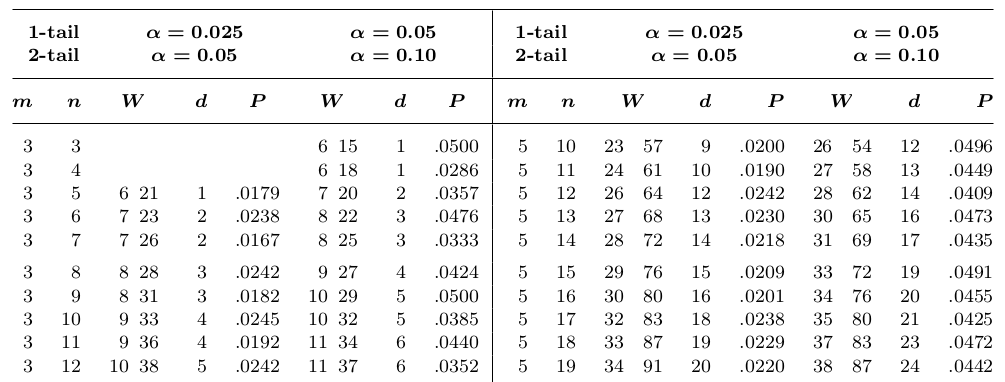
\includegraphics[width=\linewidth]{./images/rc6fig1.png}
\end{figure}
A larger table can be found in rc files.

\end{frame}


\begin{frame}{Wilcoxon Rank-Sum Test}

\justifying
\structb{Wilcoxon rank-sum test.} For large values of $m (m\geq 20)$, $W_m$ is approximated normally distributed with
\begin{align*}
\U{E}[W_m] = \frac{m(m+n+1)}{2}, \qquad \U{Var}[W_m] = \frac{mn(m+n+1)}{12}.
\end{align*}
In case of ties, the variance may be corrected by taking
\begin{align*}
\U{Var}[W_m] = \frac{mn(m+n+1)}{12-\displaystyle \sum_{\U{groups}} \frac{t^3+t}{12}},
\end{align*}
where the sum is taken over all groups of $t$ ties.


\end{frame}



\subsection{Paired Tests}


\begin{frame}{Variances Equal but Unknown --- Paired $T$-Test}

\justifying
\structb{Paired T-test.} Let $X_1^{(i)}, \ldots, X_{n_i}^{(i)}$ with $i = 1, 2$ be samples of size $n = n_1 = n_2$ from normal distributions with unknown means $\mu_1, \mu_2$ and \highlightr{equal} but \highlightr{unknown} variances $\sigma^2 = \sigma_1^2 = \sigma_2^2$. Then $D_i = X_i - Y_i$ follows normal distributions. Then the test statistic is given by
\begin{align*}
T_{n-1} = \frac{\overline{D} - \mu_0}{\sqrt{S^2_D/n}}.
\end{align*}
We reject at significance level $\alpha$
\begin{itemize}
	\item $H_0: \mu_D = \mu_0$ if $|T_{n-1}| > t_{\alpha/2,n-1}$,
	\item $H_0: \mu_D \leq \mu_0$ if $T_{n-1} > t_{\alpha,n-1}$,
	\item $H_0: \mu_D \geq \mu_0$ if $T_{n-1} < -t_{\alpha,n-1}$.
\end{itemize}


\end{frame}

\begin{frame}{Paired vs. Pooled $T$-Tests}

\justifying
With two populations $X$ and $Y$ with equal variances $\sigma^2$, we want to test $H_0: \mu_X = \mu_Y$ using samples of equal size $n$. Then the statistics are
\footnotesize
\begin{align*}
T_{\U{pooled}} & = \frac{\overline{X} - \overline{Y}}{\sqrt{2S_p^2/n}}, \qquad  \U{critical\ value} = t_{\alpha/2,2n-2}, \\
T_{\U{paired}} & = \frac{\overline{X}-\overline{Y}}{\sqrt{S_D^2/n}}, \qquad\ \U{critical\ value} = t_{\alpha/2,n-1}.
\end{align*}
\normalsize
Preferring a more powerful test, we consider the following.
\begin{itemize}
	\justifying
	\item $t_{\alpha/2,2n-2} < t_{\alpha/2,n-1}$, smaller critical values $\Rightarrow$ easier to reject.
	\item $2S_p^2/n$ estimates $2\sigma^2/n$, while $S_D^2/n$ estimates $\sigma_D^2/n = \sigma_{\overline{D}}^2$, where
	\footnotesize
	\begin{align*}
	\sigma_{\overline{D}}^2 = \frac{2\sigma^2}{n}(1-\rho_{\overline{X}\overline{Y}}) = \frac{2\sigma^2}{n}(1-\rho_{XY}).
	\end{align*}
	\normalsize
	When $\rho_{XY} > 0$, paired T-test would be more powerful.
\end{itemize}

\end{frame}


\begin{frame}{Non-parametric Paired Test}

\justifying
\structb{Comparison of medians.} Let $X$ and $Y$ be two independent random variables that follow the same distribution but differ only in their location, i.e., $X':=X-\delta$ and $Y$ are independent and identically distributed. Then $D = X - Y$ and $2\delta-D$ follow the same distribution. Therefore, $D$ is symmetric about $\delta$, .i.e.,
\begin{align*}
f_D(\delta+d) = f_D(\delta-d).
\end{align*}
Then we can perform the Wilcoxon signed-rank test on $D$.

\end{frame}


\subsection{Correlation Coefficient}

\begin{frame}{Estimating Correlation}

\structb{Estimator for correlation.} The unbiased estimators for variance and covariance are given by
\begin{align*}
\widehat{\U{Var}[X]} & = \frac{1}{n-1}\sum_{i=1}^n(X_i-\overline{X})^2, \\
\widehat{\U{Var}[Y]} & = \frac{1}{n-1}\sum_{i=1}^n(Y_i-\overline{Y})^2, \\
\widehat{\U{Cov}[X, Y]} & = \frac{1}{n-1} \sum_{i=1}^n (X_i-\overline{X})(Y_i-\overline{Y}),
\end{align*}
giving
\begin{align*}
R := \widehat{\rho} = \frac{\sum(X_i-\overline{X})(Y_i-\overline{Y})}{\sqrt{\sum(X_i-\overline{X})^2}\sqrt{\sum(Y_i-\overline{Y})^2}}.
\end{align*}

\end{frame}

\begin{frame}{Hypothesis Tests for the Correlation Coefficient}

\justifying
\structb{Distribution.} Suppose $(X, Y)$ follows a bivariate normal distribution with relation coefficient $\rho\in (-1, 1)$. For large sample size $n$, the Fisher transformation of $R$
\begin{align*}
\frac{1}{2}\ln\left(\frac{1+R}{1-R} \right) = \U{Artanh}(R) 
\end{align*}
is approximately normal with
\begin{align*}
\mu = \frac{1}{2}\ln\left(\frac{1+\rho}{1-\rho} \right) = \U{Artanh}(\rho), \qquad \sigma^2 = \frac{1}{n-3}.
\end{align*}

\end{frame}

\begin{frame}{Hypothesis Tests for the Correlation Coefficient}

\justifying
\structb{Confidence interval.} A $100(1-\alpha)\%$ confidence interval for $\rho$ is given by
\begin{align*}
\left[\frac{1+R-(1-R)e^{2z_{\alpha/2}/\sqrt{n-3}}}{1+R+(1-R)e^{2z_{\alpha/2}/\sqrt{n-3}}},  \frac{1+R-(1-R)e^{-2z_{\alpha/2}/\sqrt{n-3}}}{1+R+(1-R)e^{-2z_{\alpha/2}/\sqrt{n-3}}}\right]
\end{align*}
or
\begin{align*}
\tanh\left(\U{Artanh}(R) \pm \frac{z_{\alpha/2}}{\sqrt{n-3}} \right).
\end{align*}


\end{frame}


\begin{frame}{Hypothesis Tests for the Correlation Coefficient}

\justifying
\structb{Test for correlation coefficient.} Suppose $(X_1, Y_1), \ldots, (X_n, Y_n)$ is a sample of size $n$ from a bivariate normal population $(X, Y)$ with correlation coefficient $\rho\in (-1, 1)$. The test statistic is given by
\begin{align*}
Z & = \frac{\sqrt{n-3}}{2}\left(\ln\left(\frac{1+R}{1-R} \right) - \ln\left(\frac{1+\rho_0}{1-\rho_0} \right) \right) \\
& = \sqrt{n-3}(\U{Artanh}(R) - \U{Artanh}(\rho_0)).
\end{align*}
We reject at significance level $\alpha$
\begin{itemize}
	\item $H_0: \rho = \rho_0$ if $|Z| > z_{\alpha/2}$,
	\item $H_0: \rho \leq \rho_0$ if $Z > z_{\alpha}$,
	\item $H_0: \rho \geq \rho_0$ if $Z < -z_{\alpha}$.
\end{itemize}


\end{frame}


\section{Categorical Data}


\subsection{Categorical Data and Multinomial Distribuiton}

\begin{frame}{The Multinomial Distribution}

\justifying
\structb{Definition.} A random vector $((X_1, \ldots, X_k), f_{X_1X_2\cdots X_k})$ with 
\begin{align*}
(X_1, \ldots, X_k): S\rightarrow \Omega = \{0, 1, 2, \ldots, n\}^k
\end{align*}
and joint distribution function $f_{X_1X_2\cdots X_k}: \Omega\rightarrow\R$
\begin{align*}
f_{X_1X_2\cdots X_k}(x_1, \ldots, x_k) = \frac{n!}{x_1!\cdots x_k!} p_1^{x_1}\cdots p_k^{x_k},
\end{align*}
$p_1,\ldots, p_k\in (0, 1), n\in \N\setminus\{0\}, p_1 + \cdots + p_k = 1$ is said to have a \highlightg{multinomial distribution} with parameters $n$ and $p_1,\ldots, p_k$. For $i = 1,\ldots, k$ and $1\leq i < j\leq k$,
\begin{align*}
\U{E}[X_i] = np_i, \quad \U{Var}[X_i] = np_i(1-p_i), \quad \U{Cov}[X_i, X_j] = -np_ip_j.
\end{align*}

\end{frame}

\subsection{The Pearson Statistic}

\begin{frame}{The Pearson Statistic}

\justifying
\structb{Theorem.} Let $((X_1, \ldots, X_k), f_{X_1X_2\cdots X_k})$ be a multinomial random variable with parameters $n$ and $p_1, \ldots, p_k$. For large $n$ the \highlightg{Pearson statistic}
\begin{align*}
\sum_{i=1}^k \frac{(O_i-E_i)^2}{E_i} = \sum_{i=1}^k \frac{(X_i-np_i)^2}{np_i}
\end{align*}
follows an approximate chi-squared distribution with $k-1$ degrees of freedom, where $O_i$ are observed values and $E_i$ are expected values. \\
\structb{Cochran's rule.} For good approximation, we require
\begin{align*}
\U{E}[X_i] & = np_i \geq 1, \qquad \U{for\ all\ } i = 1, \ldots, k,\\
\U{E}[X_i] & = np_i \geq 5, \qquad \U{for\ 80\%\ of\ all\ } i = 1,\ldots, k.
\end{align*}

\end{frame}

\begin{frame}{Test for Multinomial Distribution}

\justifying
\structb{Pearson's chi-squared goodness-of-fit test.} Let $(X_1, \ldots, X_k)$ be a sample of size $n$ from a categorical random variable with parameters $p_1, \ldots, p_k$ satisfying Cochran's Rule. Let $(p_{1_0}, \ldots, p_{k_0})$ be a vector of null values. We want to test
\begin{align*}
H_0: p_i = p_{i_0}, \qquad i = 1,\ldots, k.
\end{align*}
based on the test statistic
\begin{align*}
X_{k-1}^2 = \sum_{i=1}^k \frac{(X_i - np_{i_0})^2}{np_{i_0}}.
\end{align*}
We reject $H_0$ at significance level $\alpha$ if $X_{k-1}^2 > \chi_{\alpha,k-1}^2$.

\end{frame}


\begin{frame}{Goodness-of-Fit Test for a Discrete Distribution}

\justifying
\structb{Goodness-of-fit test.} Dividing large data into $k$ categories to estimate $m$ parameters of distributions, we have the statistic
\begin{align*}
\sum_{i=1}^k \frac{(O_i - E_i)^2}{E_i}
\end{align*}
which follows a chi-squared distribution with $k-1-m$ degrees of freedom. This transforms the question of ``whether a certain variable follows some specific distribution with parameters $\theta$'' to ``whether the categorical variable follows the multinomial distribution with parameters $p_1,\ldots, p_k$ determined by the specific distribution with parameters $\theta$''.\\
\structb{Degrees of freedom.} The degrees of freedom is given by
\begin{align*}
\U{df} = \#\{\U{independent\ cells}\} - \#\{\U{estimated\ parameters}\}.
\end{align*}

\end{frame}

\begin{frame}{Test for Independence of Categorizations}

\structb{Overview.}
\begin{enumerate}
	\justifying
	\item Draw \highlightg{contingency table} from data, and calculate the marginal row and column sums.
	\begin{table}
		\footnotesize
		\centering
		\begin{tabular}{c|ccc|c}
			 & cat.2.1 & $\cdots$ & cat.2.c & \\
			\hline
			cat.1.1 & $n_{11}$ & $\cdots$ & $n_{1c}$ & $n_{1\cdot}$ \\
			$\vdots$ & $\vdots$ & $\ddots$ & $\vdots$ & $\vdots$ \\
			cat.1.r & $n_{r1}$ & $\cdots$ & $n_{rc}$ & $n_{r\cdot}$ \\
			\hline
			& $n_{\cdot 1}$ & $\cdots$ & $n_{\cdot c}$ & $n$
		\end{tabular}
	\end{table}
	\item Calculate Pearson statistic
	\footnotesize
	\begin{align*}
	X^2_{(r-1)(c-1)} = \sum_{i=1}^r \sum_{j=1}^c \frac{(O_{ij}-E_{ij})^2}{E_{ij}}, \quad \U{where\ } E_{ij} = \frac{n_{i\cdot}n_{\cdot j}}{n}.
	\end{align*}
	\normalsize
	\item Reject $H_0: p_{ij} = p_{i\cdot}p_{\cdot j}$ at significance level $\alpha$ if $X^2_{(r-1)(c-1)} > \chi_{\alpha,(r-1)(c-1)}^2$.
\end{enumerate}

\end{frame}


\begin{frame}{Test for Homogeneity}

\structb{Overview.}
\begin{enumerate}
	\justifying
	\item Draw contingency table. (Suppose the marginal row sums are fixed.)
	\begin{table}
		\footnotesize
		\centering
		\begin{tabular}{c|ccc|c}
			& cat.2.1 & $\cdots$ & cat.2.c & \\
			\hline
			cat.1.1 & $n_{11}$ & $\cdots$ & $n_{1c}$ & $n_{1\cdot}$ (fixed) \\
			$\vdots$ & $\vdots$ & $\ddots$ & $\vdots$ & $\vdots$ \\
			cat.1.r & $n_{r1}$ & $\cdots$ & $n_{rc}$ & $n_{r\cdot}$ (fixed) \\
			\hline
			& $n_{\cdot 1}$ & $\cdots$ & $n_{\cdot c}$ & $n$ (fixed)
		\end{tabular}
	\end{table}
	\item Calculate Pearson statistic
	\footnotesize
	\begin{align*}
	X^2_{(r-1)(c-1)} = \sum_{i=1}^r \sum_{j=1}^c \frac{(O_{ij}-E_{ij})^2}{E_{ij}}, \quad \U{where\ } E_{ij} = \frac{n_{i\cdot}n_{\cdot j}}{n}.
	\end{align*}
	\normalsize
	\item Reject $H_0: p_{1j} = \cdots = p_{rj}$ at significance level $\alpha$ if $X^2_{(r-1)(c-1)} > \chi_{\alpha,(r-1)(c-1)}^2$.
\end{enumerate}


\end{frame}



\begin{frame}{}

\centering
\emph{Thanks for your attention!}
%\highlightr{\\Good luck for Midterm exam!}
  
\end{frame}

\end{document}


